\subsection{Disparity Algorithm}
What is disparity
\subsubsection{Image Rectification} \label{rectsec}
The Sum of Absolute Differences algorithm operates under the assumption that objects in both camera images lie on the same horizontal line between both images, known as an epipolar line. An example of shared epipolar lines between camera imagery is shown in Figure \ref{epipolarLines} below. Although an ideal stereo camera setup would contain shared epipolar lines between camera images, raw image data from each camera will contain slight differences in object location based on the physical position of the camera modules, as well as minor differences in the lenses of each camera. Both input images can be adjusted to share the same epipolar lines through a post-processing step known as image rectification. 
\par
\begin{figure}[H]
	\centerline{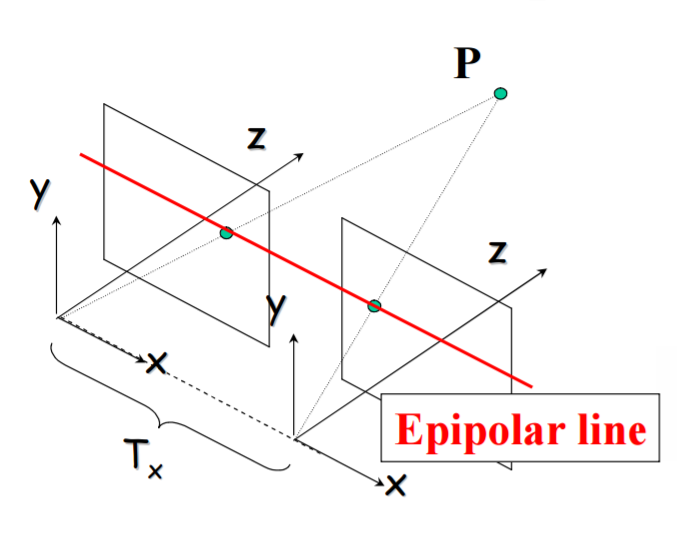
\includegraphics[width=0.75\textwidth]{epipolarLines.PNG}}
	\caption{Horizontal Epipolar Lines \cite{collins}}
	\label{epipolarLines}
\end{figure}
\par
A pictorial representation of the process of stereo image rectification is shown in Figure \ref{rectification} below \cite{mattoccia_slides}. This process is achieved using a 3x3 matrix coordinate transform based on parameters obtained from the external calibration process. 
\begin{figure}[H]
	\centerline{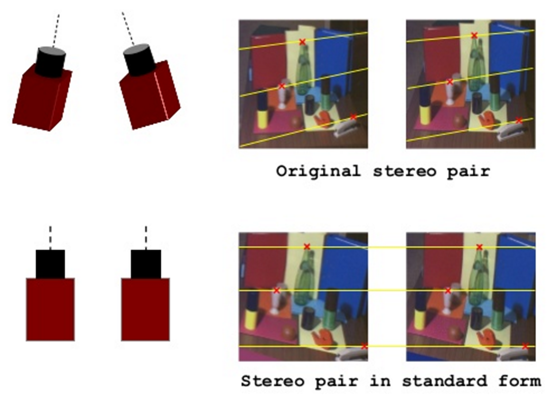
\includegraphics[width=0.75\textwidth]{rectification.png}}
	\caption{Stereo Image Rectification \cite{mattoccia_slides}}
	\label{rectification}
\end{figure}
\par
After a given pair of images has been rectified, it is then possible to perform the Sum of Absolute Differences on the given image pair in order to extract depth information. 
\subsubsection{Sum of Absolute Differences}
The method used in our disparity algorithm implementation is known as the Sum of Absolute Differences, or SAD. SAD is a common digital image processing technique used to measure the similarity between blocks of image data. In the case of our stereo camera interface, a SAD algorithm is used to search through the right image data for windowed blocks that match a template block selected from the left camera image. This process is performed using 7x7 pixel search blocks over 50 pixel horizontal ranges, and is repeated throughout the image. The expression for the sum of absolute differences is shown in Equation \ref{disparityEQN} below. 
\par
% sum(sum(abs(template-block)))
\begin{equation}\label{disparityEQN}
SAD = \sum_{x}^{}\sum_{y}^{}|template-block|
\end{equation}
\par
A visual representation of the Sum of Absolute differences is shown in Figure \ref{SAD}, with the top image showing the left image template block, and the middle image showing the right image search window in relation to the location of the template block. Below both images is a visual representation of the Sum of Absolute Differences between the template block and the current search block, outlined in white. In the case of the current search, the template and search blocks are relatively different, resulting in a high SAD value. 
\par
\begin{figure}[H]
	\centerline{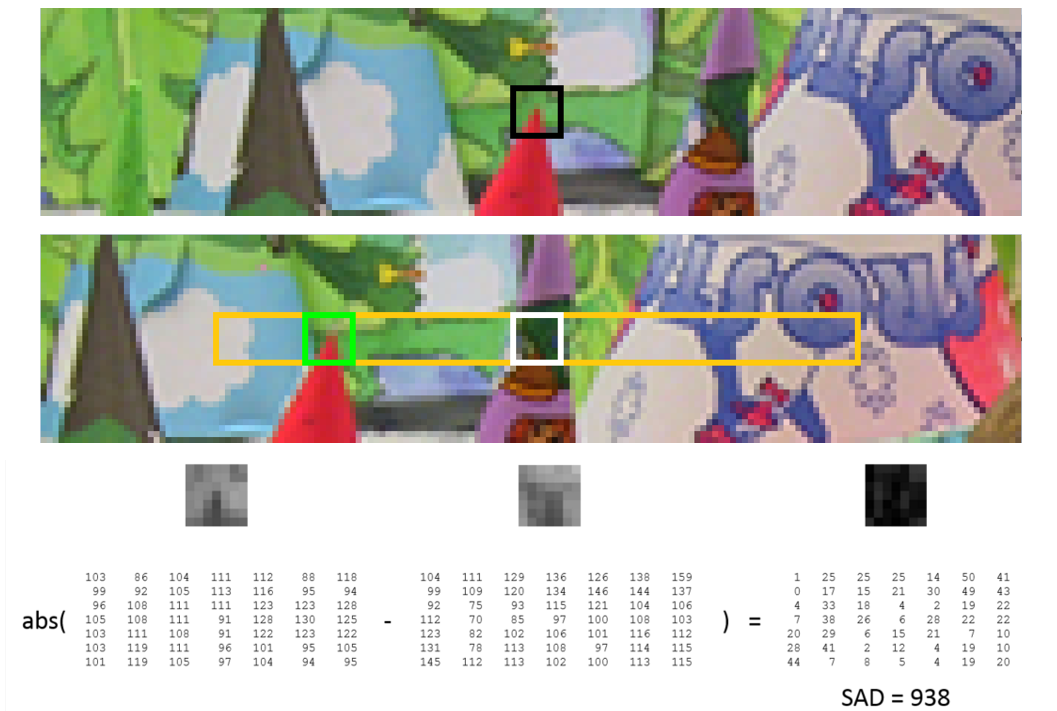
\includegraphics[width=0.75\textwidth]{SAD.PNG}}
	\caption{Sum of Absolute Differences \cite{mccormick}}
	\label{SAD}
\end{figure}
\par
Since the disparity algorithm used in this implementation calculates the sum of absolute differences for multiple search blocks, the resulting SAD values for each search block can be compared to find the location of the most similar matching block in the search image. Due to the nature of the SAD algorithm, lower SAD values indicate higher similarity between the template and search blocks. This comparison is demonstrated in Figure \ref{blockMatching} below. In the case of Figure 
\ref{blockMatching}, higher match score values for each search block indicate lower SAD values.
\par
\begin{figure}[H]
	\centerline{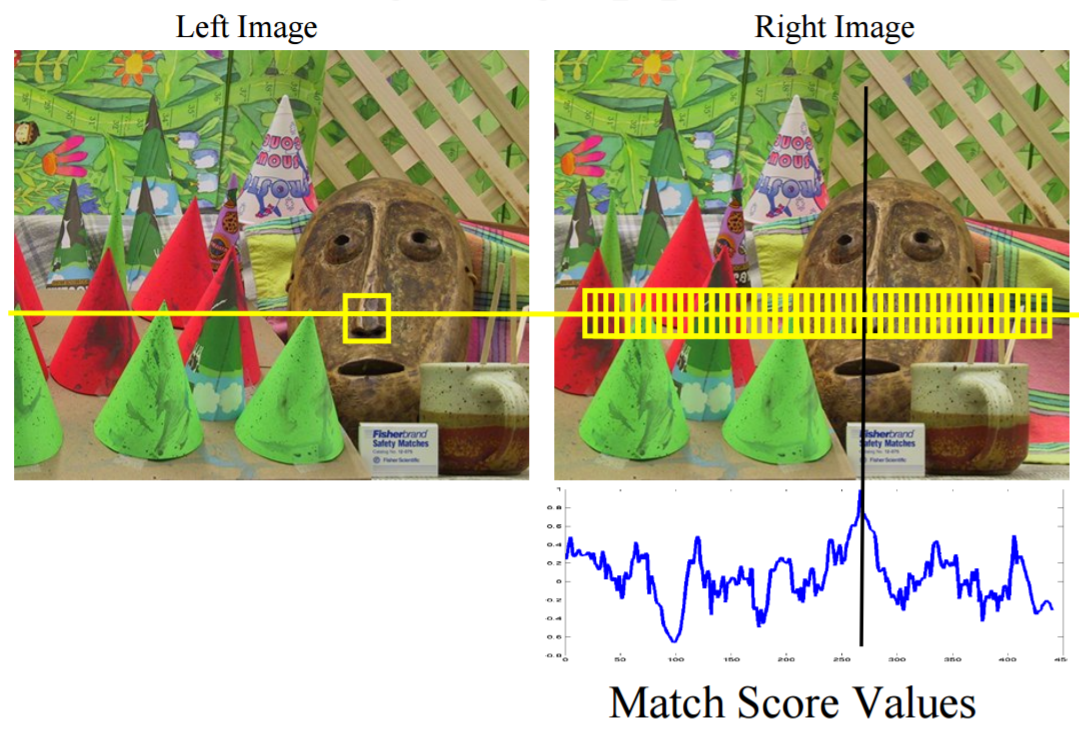
\includegraphics[width=0.75\textwidth]{blockMatching.PNG}}
	\caption{Block Matching Overview \cite{collins}}
	\label{blockMatching}
\end{figure}
\par
The SAD at multiple search points can be used to estimate the pixel offset between the template block and matching search block based on array index locations, since all SAD values for a single search are stored in a vector. This pixel offset is known as the disparity value for a given template and search block. The disparity $d$ at a given point can be transformed into a units of distance using the focal point $f$ and baseline distance $T_x$ between image sensors as shown in Equation \ref{disp2dist} below. 
\par
\begin{equation}\label{disp2dist}
depth = Z = \frac{fT_x}{d}
\end{equation}
\par
Pixel coloration values in a disparity image are based on the distance calculation shown in Equation \ref{disp2dist}, where each pixel is referenced to the disparity at a given template block's location. An example disparity image created using a given pair of test images is shown in Figure \ref{disparityOutput} below. 
\par
\begin{figure}[H]
	\centerline{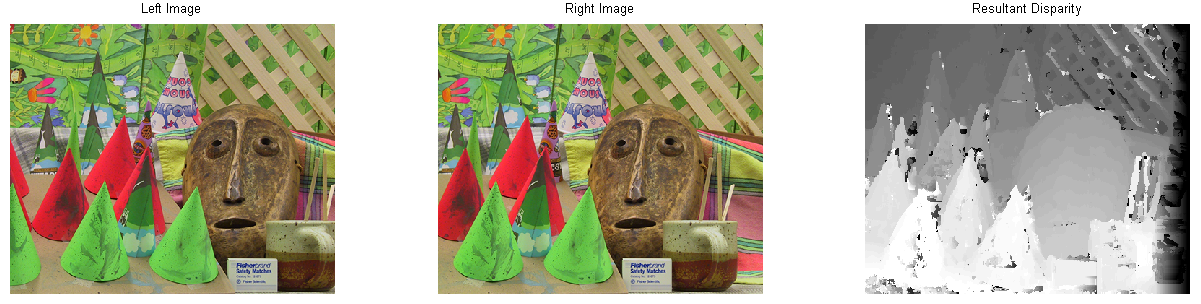
\includegraphics[width=1.1\textwidth]{disparity.png}}
	\caption{Disparity Algorithm Output}
	\label{disparityOutput}
\end{figure}